\documentclass[11pt]{article}

\usepackage[a4paper,margin=1in]{geometry}
\usepackage{amsmath,amssymb,amsthm}
\usepackage{hyperref}
\usepackage{graphicx}
\usepackage{listings}
\usepackage{algorithm}
\usepackage{algpseudocode}
\usepackage{enumitem}
\usepackage{mathtools}
\usepackage{booktabs}
\usepackage{array}
\usepackage{tikz}
\usetikzlibrary{arrows.meta,positioning,shapes.geometric}

\hypersetup{
  colorlinks=true,
  linkcolor=blue,
  urlcolor=blue,
  citecolor=blue
}

\newcommand{\version}{v1.0.2}
\newcommand{\project}{JACK}

\title{\textbf{\project: Just-in-time Autonomous Cross-chain Kernel}\\
A Formal Architecture for Intent-Based, Privacy-Aware, and Policy-Enforced DeFi Execution\\
{\large \version}
}

\author{
Blockchain Foundation LatAm\\
\texttt{research@lukas.lat}
}
\date{February 2026}

\begin{document}
\maketitle

\begin{abstract}
Liquidity, execution venues, and state have fragmented across heterogeneous blockchain ecosystems, creating a usability and safety bottleneck for decentralized finance. While bridges, aggregators, and routers enable cross-domain value movement, they do not provide a unified \emph{execution abstraction} with explicit policy enforcement and a rigorous failure model.

This paper introduces \project, a protocol-level execution kernel that transforms high-level user intents into verifiable, policy-constrained execution plans and settles them on programmable venues (e.g., Uniswap v4 hooks). \project separates (i) intent representation, (ii) solver coordination, (iii) private constraint handling, (iv) routing, and (v) settlement adapters.

\textbf{Scope note (v1).} \project~\version remains a practical, implementation-aligned specification. Private constraints are handled via a pluggable \emph{Confidential Constraint Module (CCM)} interface, while stronger FHE+ZK enforcement remains a forward-looking research direction.
\end{abstract}

\tableofcontents
\newpage

%-------------------------------------------------
\section{Versioning, Scope, and Non-Goals}

\subsection{Change Log}
\begin{itemize}
\item \textbf{v1.0.2} (Feb 2026): Adds implementation-aligned details for LI.FI quote/route/status integration, Yellow Network provider notifications/auth persistence flow, deterministic \texttt{/api/quote} semantics with explicit fallback mode, and production process diagrams.
\item \textbf{v1.0.1} (Feb 2026): Clarified v1 scope; replaced hard FHE claims with CCM interface; added explicit non-goals for cross-chain atomicity; added minimal solver economic model; expanded threat model and hook security considerations.
\item \textbf{v1.0.0} (Feb 2026): Initial formal architecture draft.
\end{itemize}

\subsection{What is in-scope for v1}
\begin{itemize}
\item Concrete intent format with public envelope and private constraints.
\item Solver competition with minimal economic security primitive (bonded execution).
\item Routing via existing infrastructure (LI.FI) with explicit failure handling and deterministic API contracts.
\item Settlement on a single destination chain using programmable venues (Uniswap v4 hooks).
\item Pluggable privacy interface (CCM) to reduce information leakage.
\item Provider event ingestion and persistence for execution observability (Yellow Network integration).
\end{itemize}

\subsection{Non-goals for v1}
\begin{itemize}
\item \textbf{Atomic cross-chain settlement} across heterogeneous finality domains.
\item \textbf{Trustless bridge security} (bridges are treated as external dependencies with allowlists and circuit breakers).
\item \textbf{Production-grade FHE+ZK} constraint proofs.
\item \textbf{Global solver decentralization guarantees} (v1 prioritizes correctness and observability).
\end{itemize}

\subsection{v1 vs. vNext}
\begin{center}
\begin{tabular}{>{\raggedright\arraybackslash}p{0.27\textwidth} p{0.32\textwidth} p{0.32\textwidth}}
\toprule
\textbf{Component} & \textbf{v1 (this document)} & \textbf{vNext (research / roadmap)} \\
\midrule
Private constraints & CCM interface; confidential execution/coprocessor possible & FHE+ZK proof-carrying constraints; threshold key mgmt \\
Cross-chain execution & Best-effort routing + explicit failure states & Stronger atomicity/dispute games/optimistic safety \\
Solver economics & Minimal bonded execution + fees & Auctions, staking, slashing, anti-collusion \\
Venue policy & Uniswap v4 hooks enforce policy & Formal verification and hook attestation registries \\
Provider telemetry & Yellow notifications and persistence & Multi-provider reconciliation and cryptographic attestations \\
\bottomrule
\end{tabular}
\end{center}

%-------------------------------------------------
\section{Introduction}

DeFi execution has moved from single-chain composability to a multi-domain environment where users must still manually choose routes, bridges, and venues. This transaction-centric model does not scale and is vulnerable to adversarial observation and manipulation~\cite{daian2020flashbots}.

\project introduces an intent-first kernel: users specify \emph{what} they want, solvers compete to provide an execution plan, and settlement-time policies are enforced on-chain (e.g., via Uniswap v4 hooks)~\cite{uniswapv4core}. The design objective is verifiable settlement with explicit failure semantics and pluggable privacy.

%-------------------------------------------------
\section{Notation and Preliminaries}

Let $\mathbb{B}=\{0,1\}$ be the Boolean domain. For probabilistic polynomial-time algorithm $A$, write $y \leftarrow A(x)$. Let $\lambda$ denote the security parameter.

We denote public-key encryption as $\mathsf{PKE}=(\mathsf{KeyGen},\mathsf{Enc},\mathsf{Dec})$, fully homomorphic encryption as $\mathsf{FHE}=(\mathsf{KeyGen},\mathsf{Enc},\mathsf{Eval},\mathsf{Dec})$, and zero-knowledge proof systems as $\mathsf{ZK}=(\mathsf{Prove},\mathsf{Verify})$.

%-------------------------------------------------
\section{System Architecture}

\project is decomposed into five orthogonal layers:

\begin{enumerate}[leftmargin=2em]
    \item \textbf{Intent Layer}
    \item \textbf{Solver and Coordination Layer}
    \item \textbf{Privacy / Constraint Layer (CCM)}
    \item \textbf{Execution Routing Layer}
    \item \textbf{Settlement Adapter Layer}
\end{enumerate}

\subsection{Kernel Model}

\[
\mathcal{K} = \langle \mathcal{I}, \mathcal{S}, \mathcal{C}, \mathcal{R}, \mathcal{V} \rangle
\]

where $\mathcal{I}$ denotes intent representation, $\mathcal{S}$ solver coordination, $\mathcal{C}$ privacy/constraint enforcement, $\mathcal{R}$ routing, and $\mathcal{V}$ settlement venues.

%-------------------------------------------------
\section{Reference Implementation Mapping (v1.0.2)}

\subsection{Control Plane and APIs}

The current implementation maps architecture layers into operational API surfaces:

\begin{center}
\begin{tabular}{>{\raggedright\arraybackslash}p{0.27\textwidth} p{0.29\textwidth} p{0.35\textwidth}}
\toprule
\textbf{Layer} & \textbf{Interface} & \textbf{Behavior in v1.0.2} \\
\midrule
Intent Layer & \texttt{/api/intents} & Create/list intents, persist lifecycle metadata, normalize execution context. \\
Routing Layer & \texttt{/api/quote} + LI.FI SDK & Deterministic quote schema, explicit fallback mode when upstream quote/route/status calls fail. \\
Provider Telemetry & Yellow provider notifications & Authenticated notification ingestion, persistence, and replay-safe lifecycle updates. \\
Settlement Layer & Adapter + hook contracts & Submit settlement transaction and verify policy constraints during execution. \\
Observability & Intent state records & Canonical state machine trace for created/quoted/executing/settled/aborted/expired. \\
\bottomrule
\end{tabular}
\end{center}

\subsection{Deterministic Quote Contract}

For a request $q$, the quote endpoint returns:
\[
\mathsf{QuoteResult}(q) = \langle \texttt{mode}, \texttt{route}, \texttt{reasonCode}, \texttt{expiresAt} \rangle
\]
where \texttt{mode} is either \texttt{provider} or \texttt{fallback}. This creates explicit downstream semantics for UI and solver behavior without silent partial failures.

%-------------------------------------------------
\section{Intent Model}

\subsection{Formal Intent Definition}

An intent is:
\[
I = \langle U, A, T, \Phi, \Omega \rangle
\]
where $U$ is user identifier, $A$ target asset set, $T$ destination execution environment, $\Phi$ private constraint payload, and $\Omega$ public execution envelope.

\subsection{Public and Private Components}

\[
I = (I_{pub}, \mathsf{Enc}(I_{priv}))
\]

In v1, encryption may be omitted depending on CCM implementation, but sensitive constraints should not be publicly broadcast in cleartext.

%-------------------------------------------------
\section{Solver-Based Execution}

\subsection{Competition Model}

For candidate plan $\pi$, the kernel verifies:
\begin{enumerate}
\item compatibility with $I_{pub}$,
\item satisfaction of constraints via CCM evidence,
\item verifiability of final settlement on venue $v$.
\end{enumerate}

\subsection{Minimal Economic Security (v1)}

\begin{itemize}
\item User signs intent with max fee and deadline.
\item Solver registers execution with bond $b$.
\item Invalid or expired execution can trigger slash path.
\item Winner receives fee after verified settlement.
\end{itemize}

%-------------------------------------------------
\section{Privacy / Constraint Layer: CCM}

\subsection{CCM Interface}

\[
\mathsf{CCM.Verify}(I_{pub}, \Phi, x) \rightarrow \mathbb{B}
\]

where $x$ are solver execution parameters (route, expected output, timing).

\subsection{Implementation Paths}
\begin{itemize}
\item Confidential execution/coprocessor with signed attestations (v1 path).
\item FHE evaluation of constraint circuits (research track)~\cite{gentry2009fhe,tfhe2020}.
\item ZK proofs over committed constraints (research track).
\end{itemize}

%-------------------------------------------------
\section{Routing and Provider Integration}

\subsection{Routing Graph}

\[
G = (V_{chains}, E_{bridges})
\]

Edges encode cost, latency, and risk. In v1, route planning is delegated to LI.FI infrastructure with protocol-side allowlists and caps~\cite{lifiDocs}.

\subsection{Yellow Notification Integration}

Yellow provider callbacks are authenticated and persisted before state transitions. This creates an append-only event trace used to reconcile provider state and API state~\cite{yellowDocs}.

\subsection{Failure Model}

Cross-domain execution is best-effort:
\[
\texttt{CREATED} \rightarrow \texttt{QUOTED} \rightarrow \texttt{EXECUTING} \rightarrow (\texttt{SETTLED} \mid \texttt{ABORTED} \mid \texttt{EXPIRED})
\]

Provider or bridge faults transition to \texttt{ABORTED} with explicit reason codes. Partial completion is not treated as atomic.

%-------------------------------------------------
\section{Settlement Adapter Layer}

Each venue $v$ implements:
\[
Execute(v, \pi) \rightarrow tx
\qquad\text{and}\qquad
Verify(v, tx) \rightarrow \mathbb{B}
\]

Uniswap v4 pools with hooks act as policy-enforced settlement venues~\cite{uniswapv4core}.

%-------------------------------------------------
\section{Process Diagrams}

\subsection{Intent Execution Lifecycle}

\begin{figure}[h!]
\centering
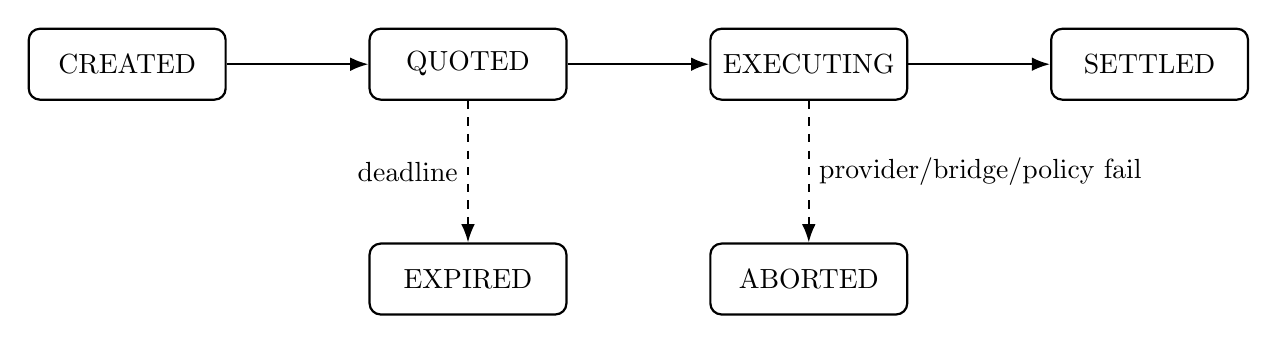
\begin{tikzpicture}[
  node distance=1.8cm,
  state/.style={rectangle, rounded corners, draw=black, thick, minimum width=2.5cm, minimum height=0.9cm, align=center},
  ok/.style={->, thick, >=Latex},
  fail/.style={->, thick, dashed, >=Latex}
]
\node[state] (created) {CREATED};
\node[state, right=of created] (quoted) {QUOTED};
\node[state, right=of quoted] (executing) {EXECUTING};
\node[state, right=of executing] (settled) {SETTLED};
\node[state, below=of executing] (aborted) {ABORTED};
\node[state, below=of quoted] (expired) {EXPIRED};

\draw[ok] (created) -- (quoted);
\draw[ok] (quoted) -- (executing);
\draw[ok] (executing) -- (settled);
\draw[fail] (executing) -- node[right]{provider/bridge/policy fail} (aborted);
\draw[fail] (quoted) -- node[left]{deadline} (expired);
\end{tikzpicture}
\caption{Canonical lifecycle enforced by JACK state transitions.}
\end{figure}

\subsection{Quote and Fallback Flow}

\begin{figure}[h!]
\centering
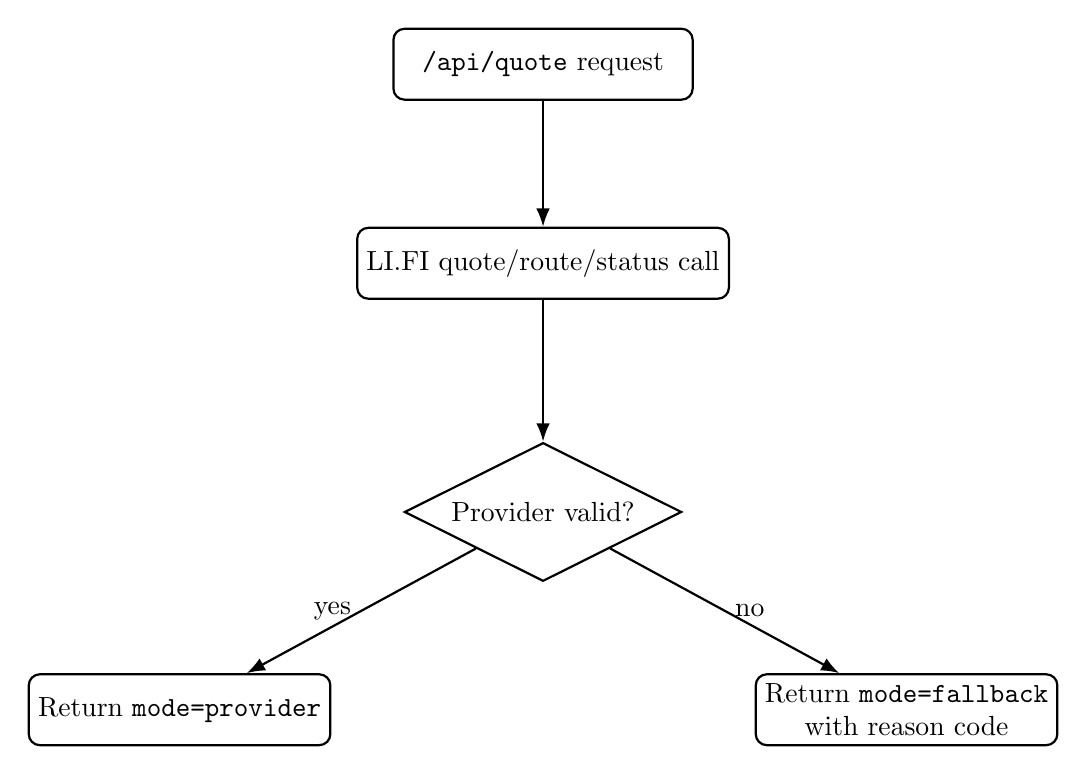
\begin{tikzpicture}[
  node distance=1.6cm,
  box/.style={rectangle, rounded corners, draw=black, thick, minimum width=3.8cm, minimum height=0.9cm, align=center},
  decision/.style={diamond, draw=black, thick, aspect=2, align=center},
  arrow/.style={->, thick, >=Latex}
]
\node[box] (request) {\texttt{/api/quote} request};
\node[box, below=of request] (provider) {LI.FI quote/route/status call};
\node[decision, below=of provider, yshift=-0.2cm] (ok) {Provider valid?};
\node[box, below left=1.6cm and 1.8cm of ok] (primary) {Return \texttt{mode=provider}};
\node[box, below right=1.6cm and 1.8cm of ok] (fallback) {Return \texttt{mode=fallback}\\with reason code};

\draw[arrow] (request) -- (provider);
\draw[arrow] (provider) -- (ok);
\draw[arrow] (ok) -- node[left]{yes} (primary);
\draw[arrow] (ok) -- node[right]{no} (fallback);
\end{tikzpicture}
\caption{Deterministic quote response behavior with explicit fallback mode.}
\end{figure}

%-------------------------------------------------
\section{Execution Algorithm}

\begin{algorithm}[H]
\caption{\project Kernel Execution (v1)}
\begin{algorithmic}[1]
\State User constructs and signs intent $I=(I_{pub}, \Phi)$
\State API stores intent and requests quote from LI.FI provider path
\State If provider quote invalid, return deterministic fallback quote result
\State Solvers submit candidate plans $\pi$ with parameters $x$
\ForAll{solver submissions}
    \State Verify public compatibility with $I_{pub}$
    \State Verify CCM evidence: $\mathsf{CCM.Verify}(I_{pub}, \Phi, x)=1$
\EndFor
\State Select winning solver $\pi^\star$ under fee and policy constraints
\State Execute routing (best-effort) and ingest Yellow provider notifications
\State Submit settlement to venue $v$ and enforce hook policy
\State Persist terminal state and emit public events
\end{algorithmic}
\end{algorithm}

%-------------------------------------------------
\section{Verification and Observability}

\subsection{Execution Correctness}

\[
\mathsf{CCM.Verify}(\cdot)=1 \;\wedge\; \mathsf{Verify}(v, tx)=1
\]

\subsection{Operational Evidence}

Observers can verify:
\begin{itemize}
\item deterministic quote mode and reason codes,
\item lifecycle transitions with persisted provider notifications,
\item settlement correctness and hook-level policy decisions.
\end{itemize}

%-------------------------------------------------
\section{Adversarial Model}

We consider:
\begin{itemize}
\item malicious solvers (invalid routes, griefing, censorship),
\item adversarial observers (MEV, timing inference),
\item routing/provider failures (outages, stale routes, auth failures),
\item malicious venue/hook logic (access control or reentrancy defects),
\item oracle manipulation affecting policy checks.
\end{itemize}

%-------------------------------------------------
\section{Security Properties (v1)}

\begin{enumerate}
\item \textbf{Policy enforceability}: settlement cannot bypass on-chain hook policy.
\item \textbf{Execution integrity}: execution is bound to signed intent and verified evidence.
\item \textbf{Fail-closed behavior}: missing evidence or policy violations abort execution.
\item \textbf{Deterministic APIs}: quote response mode is explicit and machine-checkable.
\item \textbf{Risk containment}: allowlists, caps, and circuit breakers limit blast radius.
\end{enumerate}

%-------------------------------------------------
\section{Evaluation Plan (v1.0.2)}

Measure:
\begin{itemize}
\item intent-to-settlement latency,
\item provider success vs fallback rate for \texttt{/api/quote},
\item yellow notification ingestion latency and replay rejection rate,
\item hook gas overhead and policy rejection rate,
\item route success under degraded bridge/provider conditions.
\end{itemize}

%-------------------------------------------------
\section{Limitations and Future Work}

\begin{itemize}
\item stronger economic security (auctions, staking, slashing),
\item decentralized solver participation and anti-collusion mechanisms,
\item formal verification and attestation registries for hooks,
\item cross-domain atomicity/dispute mechanisms,
\item production-ready proof-carrying private constraints.
\end{itemize}

%-------------------------------------------------
\section{Conclusion}

\project treats execution as a programmable primitive: users submit intents, solvers compete to satisfy them, routing is delegated with deterministic contracts, and on-chain venues enforce policy at settlement. Version \version aligns the specification with the implemented LI.FI and Yellow provider flows while preserving a clear path to stronger privacy and cross-domain guarantees.

\bibliographystyle{abbrv}
\begin{thebibliography}{10}

\bibitem{gentry2009fhe}
Craig Gentry.
\newblock Fully Homomorphic Encryption Using Ideal Lattices.
\newblock In \emph{Proceedings of the 41st Annual ACM Symposium on Theory of Computing (STOC)}, 2009.

\bibitem{tfhe2020}
Ilaria Chillotti, Nicolas Gama, Mariya Georgieva, and Malika Izabach{\`e}ne.
\newblock TFHE: Fast Fully Homomorphic Encryption over the Torus.
\newblock \emph{Journal of Cryptology}, 33(1), 2020.

\bibitem{daian2020flashbots}
Philip Daian, Steven Goldfeder, Tyler Kell, Yunqi Li, Xueyuan Zhao, Ittay Eyal, and Emin G{\"u}n Sirer.
\newblock Flash Boys 2.0: Frontrunning, Transaction Reordering, and Consensus Instability in Decentralized Exchanges.
\newblock In \emph{IEEE Symposium on Security and Privacy}, 2020.

\bibitem{uniswapv4core}
Uniswap Labs.
\newblock Uniswap v4 Core Architecture.
\newblock \url{https://github.com/Uniswap/v4-core}, 2024.

\bibitem{lifiDocs}
LI.FI.
\newblock LI.FI Integrator Documentation.
\newblock \url{https://docs.li.fi/}, 2026.

\bibitem{yellowDocs}
Yellow Network.
\newblock Yellow Network Provider and Notification Documentation.
\newblock \url{https://docs.yellow.org/}, 2026.

\end{thebibliography}

\end{document}
